\documentclass[12pt, titlepage]{article}

\usepackage{fullpage}
\usepackage[round]{natbib}
\usepackage{multirow}
\usepackage{booktabs}
\usepackage{tabularx}
\usepackage{graphicx}
\usepackage{float}
\usepackage{hyperref}
\hypersetup{
    colorlinks,
    citecolor=blue,
    filecolor=black,
    linkcolor=red,
    urlcolor=blue
}

%% Comments
\usepackage{color}
\newif\ifcomments\commentstrue %displays comments
%\newif\ifcomments\commentsfalse %so that comments do not display
\ifcomments
\newcommand{\authornote}[3]{\textcolor{#1}{[#3 ---#2]}}
\newcommand{\todo}[1]{\textcolor{red}{[TODO: #1]}}
\else
\newcommand{\authornote}[3]{}
\newcommand{\todo}[1]{}
\fi
\newcommand{\wss}[1]{\authornote{blue}{SS}{#1}} 
\newcommand{\plt}[1]{\authornote{magenta}{TPLT}{#1}} %For explanation of the template
\newcommand{\an}[1]{\authornote{cyan}{Author}{#1}}
%% Common Parts
\newcommand{\progname}{4TB6 - Mechatronics Capstone} % PUT YOUR PROGRAM NAME HERE
\newcommand{\authname}{Team \#5, Locked \& Loaded
\\ Abi Nevo, nevoa
\\ Elsa Bassi, bassie
\\ Steffi Ralph, ralphs1
\\ Abdul Iqbal, iqbala18
\\ Stephen De Jong, dejons1
\\ Anthony Shenouda, shenoa2} % AUTHOR NAMES                  

\usepackage{hyperref}
    \hypersetup{colorlinks=true, linkcolor=blue, citecolor=blue, filecolor=blue,
                urlcolor=blue, unicode=false}
    \urlstyle{same}


\newcounter{acnum}
\newcommand{\actheacnum}{AC\theacnum}
\newcommand{\acref}[1]{AC\ref{#1}}

\newcounter{ucnum}
\newcommand{\uctheucnum}{UC\theucnum}
\newcommand{\uref}[1]{UC\ref{#1}}

\newcounter{mnum}
\newcommand{\mthemnum}{M\themnum}
\newcommand{\mref}[1]{M\ref{#1}}

\begin{document}

\title{Module Guide for SmartLock \progname{}} 
\author{\authname}
\date{\today}

\maketitle
\thispagestyle{empty}
%\begin{figure}[h!]
  %\centering
  %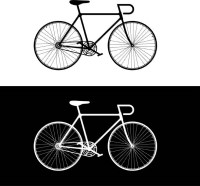
\includegraphics[width=0.4\linewidth]{../BikeLogo.jpg}
%\end{figure}
\pagenumbering{roman}

\begin{table}[hp]
\caption{Revision History} \label{TblRevisionHistory}
\begin{tabularx}{\textwidth}{p{2cm}p{3cm}X}
\toprule {\bf Date} & {\bf Developer} & {\bf Changes}\\
\midrule
02-01-23 & Elsa & Likely and Unlikely Changes \\
10-01-23 & Elsa & Modules \\
15-01-23 & Elsa & Remaining Contents \\
16-01-23 & Elsa & References \\
02-03-23 & Abi & Rev 1 Revisions--Modules reworked \\
\bottomrule
\end{tabularx}
\end{table}
\newpage

\section{Reference Material}

This section records information for easy reference.

\subsection{Abbreviations and Acronyms}

\renewcommand{\arraystretch}{1.2}
\begin{tabular}{l l} 
  \toprule		
  \textbf{symbol} & \textbf{description}\\
  \midrule 
  AC & Anticipated Change\\
  DAG & Directed Acyclic Graph \\
  M & Module \\
  MG & Module Guide \\
  OS & Operating System \\
  R & Requirement\\
  SRS & Software Requirements Specification\\
  \progname & Explanation of program name\\
  UC & Unlikely Change \\
  \bottomrule
\end{tabular}\\

\newpage

\tableofcontents

\listoftables

\listoffigures

\newpage

\pagenumbering{arabic}

\section{Introduction}

Decomposing a system into modules is a commonly accepted approach to developing
software.  A module is a work assignment for a programmer or programming
team (Parnas et al, 1984).  We advocate a decomposition
based on the principle of information hiding (Parnas, 1972a).  This
principle supports design for change, because the ``secrets'' that each module
hides represent likely future changes.  Design for change is valuable in SC,
where modifications are frequent, especially during initial development as the
solution space is explored.  

Our design follows the rules layed out by Parnas et Al (1984), as follows:
\begin{itemize}
\item System details that are likely to change independently should be the
  secrets of separate modules.
\item Each data structure is implemented in only one module.
\item Any other program that requires information stored in a module's data
  structures must obtain it by calling access programs belonging to that module.
\end{itemize}

After completing the first stage of the design, the Software Requirements
Specification (\href{https://github.com/NevoAbigail/Capstone/blob/main/docs/SRS/SRS.pdf}{SRS}), the Module Guide (MG) is developed, (Parnas et Al, 1984). The MG
specifies the modular structure of the system and is intended to allow both
designers and maintainers to easily identify the parts of the software.  The
potential readers of this document are as follows:

\begin{itemize}
\item New project members: This document can be a guide for a new project member
  to easily understand the overall structure and quickly find the
  relevant modules they are searching for.
\item Maintainers: The hierarchical structure of the module guide improves the
  maintainers' understanding when they need to make changes to the system. It is
  important for a maintainer to update the relevant sections of the document
  after changes have been made.
\item Designers: Once the module guide has been written, it can be used to
  check for consistency, feasibility, and flexibility. Designers can verify the
  system in various ways, such as consistency among modules, feasibility of the
  decomposition, and flexibility of the design.
\end{itemize}

The rest of the document is organized as follows. Section
\ref{SecChange} lists the anticipated and unlikely changes of the software
requirements. Section \ref{SecMH} summarizes the module decomposition that
was constructed according to the likely changes. Section \ref{SecConnection}
specifies the connections between the software requirements and the
modules. Section \ref{SecMD} gives a detailed description of the
modules. Section \ref{SecTM} includes two traceability matrices. One checks
the completeness of the design against the requirements provided in the SRS. The
other shows the relation between anticipated changes and the modules. Section
\ref{SecUse} describes the use relation between modules.

\section{Anticipated and Unlikely Changes} \label{SecChange}

This section lists possible changes to the system. According to the likeliness
of the change, the possible changes are classified into two
categories. Anticipated changes are listed in Section \ref{SecAchange}, and
unlikely changes are listed in Section \ref{SecUchange}.

\subsection{Anticipated Changes} \label{SecAchange}

Anticipated changes are the source of the information that is to be hidden
inside the modules. Ideally, changing one of the anticipated changes will only
require changing the one module that hides the associated decision. The approach
adapted here is called design for
change.

\begin{description}
\item[\refstepcounter{acnum}\actheacnum\label{acInput}:] The format of the initial input data and parameters on the App. 
\item[\refstepcounter{acnum}\actheacnum\label{acOutput}:] The format of the output data on the App. 
%\item[\refstepcounter{acnum}\actheacnum\label{acEngage}:] The implementation of the %transmission of the lock status signal (engaged status signal). 
\item[\refstepcounter{acnum}\actheacnum\label{acWireless}:] The implementation of the transmission of the ‘disengage’ signal. 
\item[\refstepcounter{acnum}\actheacnum\label{acBatteryStatus}:] How the battery status calculation is defined within the App. 
\item[\refstepcounter{acnum}\actheacnum\label{acPowerSignal}:] How the Arduino allows/disallows power to the load (solenoid) I.e., the implementation of the switch (transistor). 
\item[\refstepcounter{acnum}\actheacnum\label{acGeocaching}:] The implementation of the location determinant feature. 
\item[\refstepcounter{acnum}\actheacnum\label{acBattery}:] The size of the battery. 
\item[\refstepcounter{acnum}\actheacnum\label{acMagnet}:] The size of the solenoid. 
\item[\refstepcounter{acnum}\actheacnum\label{acLockingMechanism}:] The implementation of the locking mechanism. 
\item[\refstepcounter{acnum}\actheacnum\label{acLockFrame}:] The implementation of the lock frame. 

\end{description}

\subsection{Unlikely Changes} \label{SecUchange}

The module design should be as general as possible. However, a general system is
more complex. Sometimes this complexity is not necessary. Fixing some design
decisions at the system architecture stage can simplify the software design. If
these decision should later need to be changed, then many parts of the design
will potentially need to be modified. Hence, it is not intended that these
decisions will be changed.

\begin{description}

\item[\refstepcounter{ucnum}\uctheucnum\label{ucIO}:] The I/O devices (iPhone or android smartphone). 
\item[\refstepcounter{ucnum}\uctheucnum\label{ucCircuit}:] Use of the Arduino Nano BLE board, and use of a transistor and solenoid.
\item[\refstepcounter{ucnum}\uctheucnum\label{ucOutput}:] Output data are displayed to the output device (App). 
\item[\refstepcounter{ucnum}\uctheucnum\label{ucVerify}:] Output data can be verified by checking the lock frame. 
\item[\refstepcounter{ucnum}\uctheucnum\label{ucGoal}:] The goal of the system (wirelessly and hands-free disengage the bike lock). 
\item[\refstepcounter{ucnum}\uctheucnum\label{ucInput}:] There will always be a source of input data external to the software.

\end{description}

\section{Module Hierarchy} \label{SecMH}

This section provides an overview of the module design. Modules are summarized
in a hierarchy decomposed by secrets in Table \ref{TblMH}. The modules listed
below, which are leaves in the hierarchy tree, are the modules that will
actually be implemented.

\begin{description}
\item [\refstepcounter{mnum} \mthemnum \label{mUIP}:] User Input to Phone Module
\item [\refstepcounter{mnum} \mthemnum \label{mSA}:] Solenoid Actuation Module
%\item [\refstepcounter{mnum} \mthemnum \label{mESS}:] Engage Status Signal Module 
\item [\refstepcounter{mnum} \mthemnum \label{mABC}:] Arduino Bluetooth Communication Module
\item [\refstepcounter{mnum} \mthemnum \label{mMABC}:] Mobile App Bluetooth Communication Module
\item [\refstepcounter{mnum} \mthemnum \label{mBS}:] Battery Status Module 
\item [\refstepcounter{mnum} \mthemnum \label{mUD}:] User Disengage Module
\item [\refstepcounter{mnum} \mthemnum \label{mHD}:] Hardware Disengage
\item [\refstepcounter{mnum} \mthemnum \label{mL}:] Location Module 
\item [\refstepcounter{mnum} \mthemnum \label{mB}:] Battery Module 
\item [\refstepcounter{mnum} \mthemnum \label{mLM}:] Locking Mechanism Module 
\item [\refstepcounter{mnum} \mthemnum \label{mLF}:] Lock Frame Module 

\end{description}

\begin{table}[h!]
\centering
\begin{tabular}{p{0.3\textwidth} p{0.6\textwidth}}
\toprule
\textbf{Level 1} & \textbf{Level 2}\\
\midrule

\multirow{2}{0.3\textwidth}{Hardware-Hiding Module} & User Input to Phone Module \\
& Solenoid Actuation Module \\
\midrule

\multirow{6}{0.3\textwidth}{Behaviour-Hiding Module} %& Engage Status Signal Module  \\
& Arduino Bluetooth Communication Module\\
& Mobile App Bluetooth Communication Module\\
& Battery Status Module \\
& Location Module  \\
& Lock Frame Module \\
\midrule

\multirow{5}{0.3\textwidth}{Software Decision Module} & User Disengage Module \\
& Hardware Disengage Module \\
& Battery Module \\
& Locking Mechanism Module \\
\bottomrule

\end{tabular}
\caption{Module Hierarchy}
\label{TblMH}
\end{table}

\section{Connection Between Requirements and Design} \label{SecConnection}

The design of the system is intended to satisfy the requirements developed in
the \href{https://github.com/NevoAbigail/Capstone/blob/main/docs/SRS/SRS.pdf}{SRS}. In this stage, the system is decomposed into modules. The connection
between requirements and modules is listed in Table~\ref{TblRT}.

\section{Module Decomposition} \label{SecMD}

Modules are decomposed according to the principle of ``information hiding''
proposed by Parnas et al, (1984). The \emph{Secrets} field in a module
decomposition is a brief statement of the design decision hidden by the
module. The \emph{Services} field specifies \emph{what} the module will do
without documenting \emph{how} to do it. For each module, a suggestion for the
implementing software is given under the \emph{Implemented By} title. If the
entry is \emph{OS}, this means that the module is provided by the operating
system or by standard programming language libraries.  \emph{\progname{}} means the
module will be implemented by the \progname{} software.

Only the leaf modules in the hierarchy have to be implemented. If a dash
(\emph{--}) is shown, this means that the module is not a leaf and will not have
to be implemented.

\subsection{Hardware Hiding Modules}

\begin{description}
\item[Secrets:]The data structure and algorithm used to implement the virtual
  hardware.
\item[Services:]Serves as virtual hardware used by the rest of the system. This module provides the interface between the hardware and the software. So, the system can use it to display outputs or accept inputs.
\item[Implemented By:]--
\end{description}

\subsubsection{User Input to Phone Module  (\mref{mUIP})}
\begin{description}
\item[Secrets:]How the mobile app reacts to user’s touch at any point.
\item[Services:]Allows user to interface with the mobile app via touch.
\item[Implemented By:] Phone OS
\end{description}

\subsubsection{Solenoid Actuation Module  (\mref{mSA})}
\begin{description}
\item[Secrets:]Logic and implementation of the solenoid actuation depending on signal sent from Arduino.
\item[Services:]Actuates the solenoid when appropriate signal is sent from Arduino.
\item[Implemented By:] Circuit
\end{description}

\subsection{Behaviour-Hiding Module}

\begin{description}
\item[Secrets:]The contents of the required behaviours.
\item[Services:]Includes programs that provide externally visible behaviour of
  the system as specified in the software requirements specification (SRS)
  documents. This module serves as a communication layer between the
  hardware-hiding module and the software decision module. The programs in this
  module will need to change if there are changes in the SRS.
\item[Implemented By:] --
\end{description}


\subsubsection{Arduino Bluetooth Communication Module (\mref{mABC})}
\begin{description}
\item[Secrets:]Creation of infrastructure for Bluetooth communication on Arduino, searches for central device to connect to, and can successfully connect to a central device.
\item[Services:]Allows delivery of Bluetooth signals from the central connected device. 
\item[Implemented By:] Arduino
\end{description}

\subsubsection{Mobile App Bluetooth Communication and User Disengage Module (\mref{mMABC})}
\begin{description}
\item[Secrets:]Creation of infrastructure for Bluetooth communication on the app, searches for peripheral devices to connect to, and can then successfully connect to a peripheral device. Also transmits disengage signal.
\item[Services:]Allows sending of Bluetooth signals to the connected peripheral device. Then, upon pressing “Disengage” button on app, app sends required signal to peripheral device.
\item[Implemented By:] App
\end{description}

\subsubsection{Battery Status Module (\mref{mBS})}
\begin{description}
\item[Secrets:]The determination of the current level of the battery to inform the user when replacement is required.
\item[Services:]The battery level is calculated within the App based on some inherent battery properties. It is then displayed on the GUI as ‘Battery Status’. 
\item[Implemented By:]App
\end{description}

\subsubsection{Location Module (\mref{mL})}
\begin{description}
\item[Secrets:]The implementation of the location determinant.
\item[Services:]The algorithm that governs the geocaching of the bike’s location upon locking.
\item[Implemented By:]App
\end{description}

\subsubsection{Lock Frame Module (\mref{mLF})}
\begin{description}
\item[Secrets:]The design of the physical ‘lock frame’ that connects the bike and the external frame it is being ‘locked’ to.
\item[Services:]Is the interface that connects the user, the App and the locking mechanism that allows the user to utilize the entire system.
\item[Implemented By:]Mechanical System
\end{description}

\subsection{Electrical/Mechanical/Software Decision Module}

\begin{description}
\item[Secrets:] The design decision based on mathematical theorems, physical
  facts, or programming considerations. The secrets of this module are
  \emph{not} described in the SRS.
\item[Services:] Includes data structure and algorithms used in the system that
  do not provide direct interaction with the user. 
  % Changes in these modules are more likely to be motivated by a desire to
  % improve performance than by externally imposed changes.
\item[Implemented By:] --
\end{description}

\subsubsection{Hardware Disengage Module(\mref{mHD})}
\begin{description}
\item[Secrets:] Logic of HIGH and LOW signal sent from Arduino.
\item[Services:]The implementation, logic and transmission of the power signal sent from the 
the Arduino to the transistor, which acts as a switch to give power to the solenoid. 
\item[Implemented By:]Arduino
\end{description}

\subsubsection{Battery Module (\mref{mB})}
\begin{description}
\item[Secrets:]The specifications of the circuit power supply.
\item[Services:]The type and size of the battery which supplies power to the Arduino and the electromagnet. 
\item[Implemented By:]Electrical Circuit
\end{description}


\subsubsection{Locking Mechanism Module (\mref{mLM})}
\begin{description}
\item[Secrets:]The design of the moving part that engages and disengages the lock frame.
\item[Services:]Responds to the magnetic force supplied by the electromagnet in such a way that it engages and disengages the lock frame.
\item[Implemented By:]Mechanical System
\end{description}

\section{Traceability Matrix} \label{SecTM}

This section shows two traceability matrices: between the modules and the
requirements and between the modules and the anticipated changes.

% the table should use mref, the requirements should be named, use something
% like fref --> individual FR's
\begin{table}[H]
\centering
\begin{tabular}{p{0.2\textwidth} p{0.6\textwidth}}
\toprule
\textbf{Req.} & \textbf{Modules}\\
\midrule
FR1 & \mref{mUIP}, \mref{mSA}, \mref{mABC}, \mref{mMABC}, \mref{mLM}\\
FR2 & \mref{mL}\\
FR3 & \mref{mLM}\\
FR4 & \mref{mABC}, \mref{mMABC}\\
FR5 & \mref{mLF}\\
FR6 & \mref{mB}, \mref{mBS}\\
FR7 & \mref{mL}\\
FR8 & \mref{mLF}\\
\bottomrule
\end{tabular}
\caption{Trace Between Requirements and Modules}
\label{TblRT}
\end{table}

\begin{table}[H]
\centering
\begin{tabular}{p{0.2\textwidth} p{0.6\textwidth}}
\toprule
\textbf{AC} & \textbf{Modules}\\
\midrule
\acref{acInput} & \mref{mUIP}\\
\acref{acOutput} & \mref{mMABC}\\
%\acref{acEngage} & \mref{mESS}\\
\acref{acWireless} & \mref{mHD}\\
\acref{acBatteryStatus} & \mref{mBS}\\
\acref{acPowerSignal} & \mref{mHD}\\
\acref{acGeocaching} & \mref{mL}\\
\acref{acBattery} & \mref{mB}\\
\acref{acMagnet} & \mref{mSA}\\
\acref{acLockingMechanism} & \mref{mLM}\\
\acref{acLockFrame} & \mref{mLF}\\
\bottomrule
\end{tabular}
\caption{Trace Between Anticipated Changes and Modules}
\label{TblACT}
\end{table}

\section{Use Hierarchy Between Modules} \label{SecUse}

In this section, the uses hierarchy between modules is
provided. Parnas, (1978), said of two programs A and B that A {\em uses} B if
correct execution of B may be necessary for A to complete the task described in
its specification. That is, A {\em uses} B if there exist situations in which
the correct functioning of A depends upon the availability of a correct
implementation of B.  Figure \ref{FigUH} illustrates the use relation between
the modules. It can be seen that the graph is a directed acyclic graph
(DAG). Each level of the hierarchy offers a testable and usable subset of the
system, and modules in the higher level of the hierarchy are essentially simpler
because they use modules from the lower levels.

\begin{figure}[H]
\centering
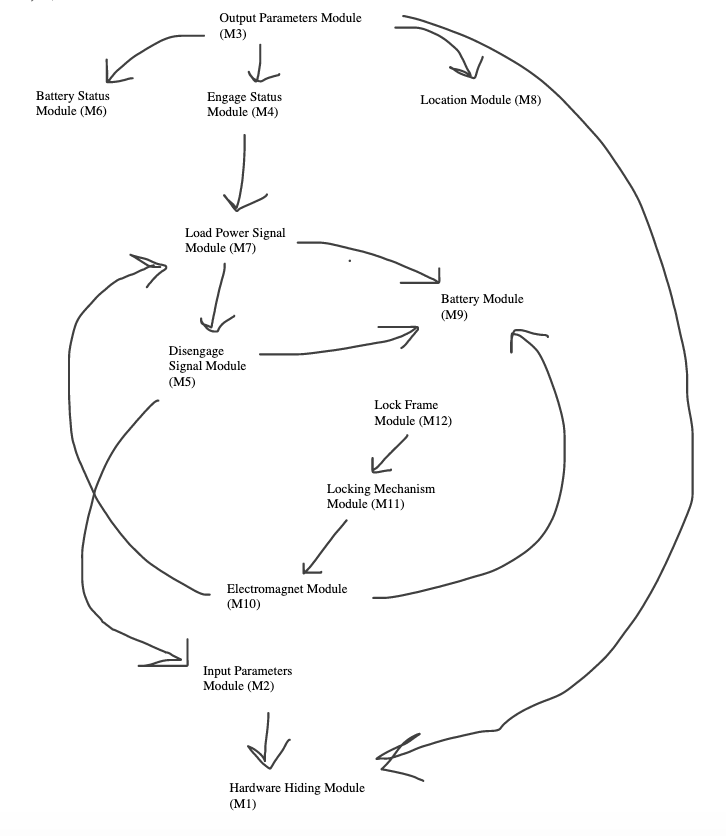
\includegraphics[width=1\textwidth]{DAG.png}
\caption{Use Hierarchy Among Modules}
\label{FigUH}
\end{figure}

%\section*{References}

\bibliographystyle {plainnat}
\bibliography{../../../refs/References}

\newpage{}

\end{document}